\documentclass{article} % For LaTeX2e
\usepackage{nips15submit_e,times}
\usepackage{amsmath}
\usepackage{amsfonts}
\usepackage{hyperref}
\usepackage{url}
\usepackage{graphicx}
\usepackage[flushleft]{threeparttable}
%\documentstyle[nips14submit_09,times,art10]{article} % For LaTeX 2.09

\usepackage{array}
\newcolumntype{L}[1]{>{\raggedright\let\newline\\\arraybackslash\hspace{0pt}}m{#1}}
\newcolumntype{C}[1]{>{\centering\let\newline\\\arraybackslash\hspace{0pt}}m{#1}}
\newcolumntype{R}[1]{>{\raggedleft\let\newline\\\arraybackslash\hspace{0pt}}m{#1}}

\title{Breast Cancer Recurrence Prediction}


\author{
Chang Liu\\
College of Engineering\\
Carnegie Mellon University\\
Pittsburgh, PA 15213 \\
\texttt{cliu5@andrew.cmu.edu} \\
\And
Kangning Chen \\
Tepper Business School \\
Carnegie Mellon University\\
Pittsburgh, PA 15213 \\
\texttt{kangninc@tepper.cmu.edu} \\
}

% The \author macro works with any number of authors. There are two commands
% used to separate the names and addresses of multiple authors: \And and \AND.
%
% Using \And between authors leaves it to \LaTeX{} to determine where to break
% the lines. Using \AND forces a linebreak at that point. So, if \LaTeX{}
% puts 3 of 4 authors names on the first line, and the last on the second
% line, try using \AND instead of \And before the third author name.

\newcommand{\fix}{\marginpar{FIX}}
\newcommand{\new}{\marginpar{NEW}}

\nipsfinalcopy % Uncomment for camera-ready version

\begin{document}


\maketitle
\begin{abstract}
Breast cancer is considered to be the second leading cause of cancer deaths in women today. Nowadays, as the development on machine technique, the data mining skills are widely used in medical industry to effectively predict and diagnosis diseases, including cancer-curing. In this essay, we will use semi-supervised machine learning to study the probability and time gaps for the potential recurrence. 
\end{abstract}

\section{Introduction}
Breast cancer is the most common cancer among women excluding non-melanoma skin cancers. Occasionally, breast cancer can return after primary treatment. Consequently, the main problem under these circumstances is to predict such a recurrent event, because only expertise from experience is not enough. 

\section{Dataset and Preprocessing}
We use two datasets for this project. The first Wisconsin Prognostic Breast Cancer (WPBC) data set contains 198 instances labeled for recurrence of breast cancer. Along with the label for recurrence, this data set records the time before recurrence or the time when a patient remains disease free. Along with the recurrence and time, this data set contains 10 relevant attributes describing the characteristics of the cell nuclei present in the digitized image of a fine needle aspirate (FNA) of the breast mass. The second Wisconsin Diagnostic Breast Cancer (WDBC) dataset contains 569 instances with the ID number and the diagnosis outcome (malign or benign) and the same 10 relevant attributes as the prognostic dataset. Each attribute has three values: The mean, standard error, and "worst" or largest. In addition, the prognostic dataset has more attributes: Time, Tumour size and Lymph node status. The detailed information is displayed in Table 1.
	
	As we mentioned, in the second dataset, WDBC, contains 569 instances unlabeled data points. However, 177 of them can be found in the WPBC data through ID matching. The matching rule is that if a WDBC ID is a prefix of a WPBC ID, then the two records are referring the same patient. Thus, one more important data feature in WPBC (malign or benign) can be added into the labelled data set WPBC.
	
	\begin{figure} 
  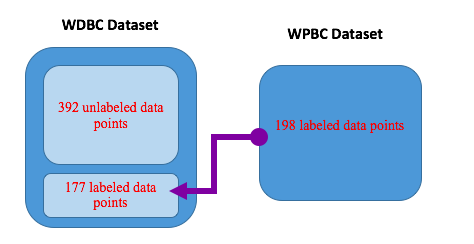
\includegraphics[width=\textwidth]{DataGraph.png}
\end{figure}

	The data set relatively clean and complete. However, we need to do two steps before implement our data. The first step is to fill the missing data. There are a few unobservable values in the attribute Lymph node status of Prognostic DataSet. We simply use the mean of the given field. 

	\begin{threeparttable}[h]
  		\centering
  		\caption{The main characteristics of the Wisconsin breast cancer dataset}
  		\label{tab:table2}
  		\begin{tabular}{| L{8cm} | c |}
		\hline
    		Attribute & Range\\
    		\hline \hline
		*Time (recurrence time if field 2 = R, disease-free time if field 2 = N) 
4-33) & (1,125)\\
		\hline
		Radius (mean of distances from the centre to all points on the perimeter ) & (10.95, 27.22)\\
		\hline
		Texture (standard deviation of gray-scale values) & (10.38, 39.28)  \\
		\hline
		Perimeter & (71.90,182.10) \\
		\hline
		Area & (361.60, 2250) \\ 
		\hline
		Smoothness (local variation in radius lengths) & (0.075, 0.145) \\
		\hline
		Compactness ($\text{perimeter}^2/\text{area}-1.0$) & (0.046, 0.311) \\
		\hline
		Concavity (severity of concave portions of the con- tour) & (0.024, 0.427) \\
		\hline
		Concave points (number of concave portions of the contour) & (0.020, 0.201) \\
		\hline
		Symmetry & (0.131, 0.304) \\
		\hline
		Fractal dimension ("coastline approximation" - 1) & (0.050, 0.097) \\
		\hline
		*Tumour size - diameter of the excised tumour in centimetres & (0.400, 10.00) \\
		\hline
		*Lymph node status - number of positive auxiliary lymph nodes & (0, 27)\\
		\hline
  		\end{tabular} 
		\begin{tablenotes}
      \small
      \item The attributes with * are the attributes that only Prognostic Dataset has.
    \end{tablenotes}
	\end{threeparttable}

\section{Methods}
\subsection{Baseline}
In {\it Diana's} paper, it uses Wisconsin Prognostic Breast Cancer dataset as the training data and apply Naive Bayesian classification on this fully labeled dataset. This methodology can serve as the baseline of our work with a testing accuracy of 74.24\%, but we may experiment on prospect of improving the accuracy by including unlabeled instances. More importantly, sensitivity and specificity should be concerned as other baseline accuracy besides the testing accuracy ($27.78\%$ and $91.67\%$ in {\it Diana's} paper). Also, we will try to implement the semi-supervised classifier by merging a supervised classifier (i.e. SVM) and an unsupervised classifier(i.e. K-means clustering) introduced in {\it D.�Rajakumari's} paper.�

\begin{figure}[!htb]
\centering
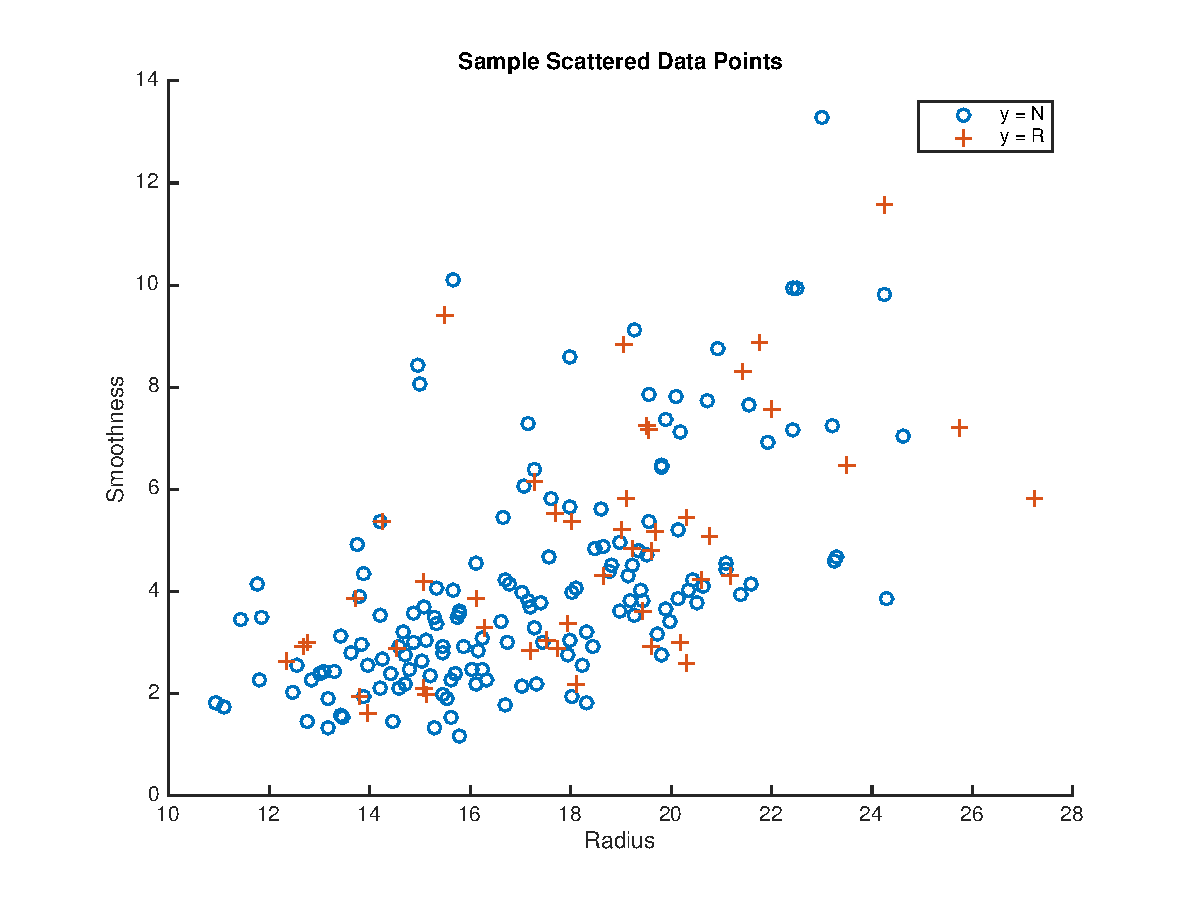
\includegraphics[scale=.7]{sampledata.eps}
\caption{Sample Graph}
\end{figure}


\subsection{First Approach: Supervised Learning}
	
\subsubsection{Gaussian Naive Bayes}
	Gaussian Naive Bayes is the methodology introduced in the {\it Diana's} paper. The essence of this methodology is to model the generative distribution of $(X, Y)$ based on the training set, and predict the outcome by choosing the highest possible label. Despite its name and its naive intuition, it is still one of the most effective and efficient algorithms for data mining. \\
	
	Naive Bayesian Classifier learns the conditional probability of each attributes $X_k$ given the class label $Y$. After that, by applying Bayes Rule, the conditional probability of $Y$ given the attributes can be computed and then we can predict $\hat{Y}$ by choosing the maximum. \\
	
	Notice that the data type of each attribute is the numerical number. The following qqplots suggest that their distribution can be well fit by Gaussian Distribution. Hence we can assume the probability density function is :
	\begin{equation*}
		\mathbb{P}(X_i|Y=y_k) = \frac{1}{\sqrt{2\pi}\sigma_{ik}}e^{-\frac{(X_i-\mu_{ik})^2}{2\sigma_{ik}^2}}
	\end{equation*}
	\begin{center}
   		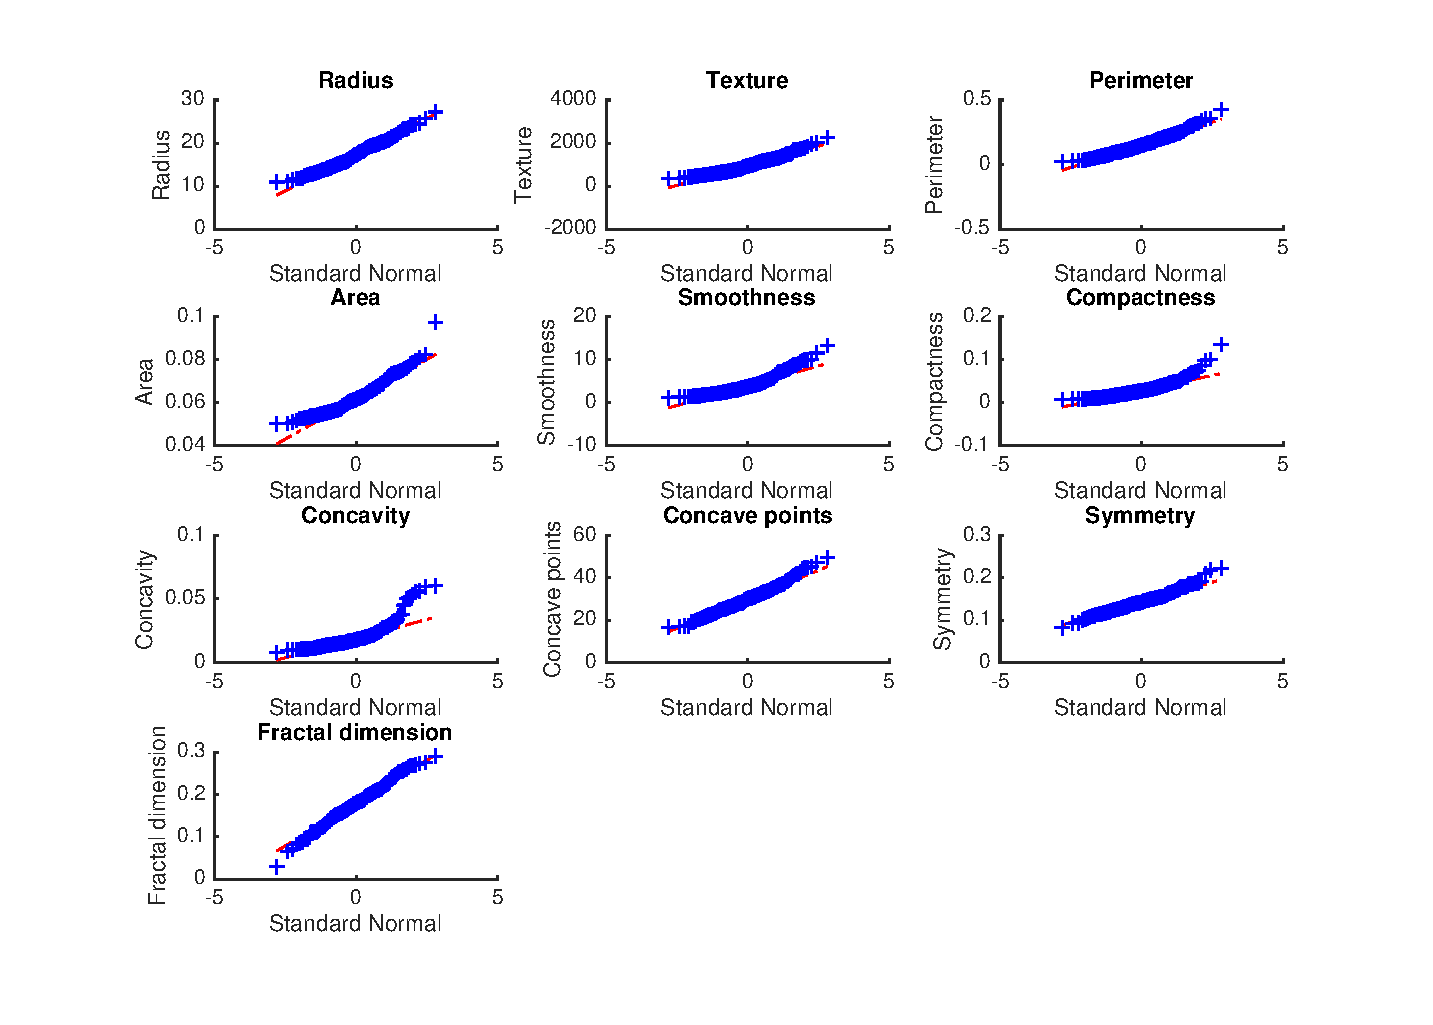
\includegraphics[scale=0.6]{DataQQPlots.eps}
	\end{center}
	
	{\it Gaussian Naive Bayes algorithm} \\
	1. Estimate $\mu_{ik} = \text{mean of $X_i$ given $Y = Y_k$}$, and $\sigma_{ik}^2 = \text{variance of $X_i$ given $Y = Y_k$}$. Also, from training set, we can estimate $\mathbb{P}(Y=y_k) = \frac{\text{number of records with }Y = y_k}{\text{sample size}}$ \\
	2. By applying bayesian rule, we want to compute: \\
	\begin{equation*}
		\mathbb{P}(Y=y_k|X=x) = \frac{\mathbb{P}(x|y_k) \mathbb{P}(y_k)}{\mathbb{P}(x)}
	\end{equation*}
	Since $\mathbb{P}(x)$ is the same for all $y_k$, we have: 
	\begin{align*}
		\hat{Y} &= argmax_{y} \frac{\mathbb{P}(x|y) \mathbb{P}(y)}{\mathbb{P}(x)}\\
			&= argmax_{y} \mathbb{P}(x|y) \mathbb{P}(y)
	\end{align*}
	3. Assume that the attributes are independent Gaussian distributed. Then: 
	\begin{equation*}
		\mathbb{P}(x|y) = \prod_i \mathbb{P}(X_i = x_i |y) = \prod_i \frac{1}{\sqrt{2\pi}\sigma_{ik}}e^{-\frac{(X_i-\mu_{ik})^2}{2\sigma_{ik}^2}}
	\end{equation*}
	4. Plug the results in step 3 back to the formula in step 2. We can compute our prediction $\hat{Y}$
	
\subsubsection{Improvements}
	We can improve the Naive Bayesian by a couple of ways. Firstly, in the methodology introduced in the {\it Diana's} paper. The Naive Bayesian assumed independence of the attributes. However, this assumption is obviously wrong. For example, Compactness = $\text{perimeter}^2/\text{area}-1.0$, which means the two attributes are highly correlated by other two fields. Also, in the training set, $corr(\text{Radius}, \text{Texture}) = 0.9929$ which is highly correlated. We can resolve this issue by applying Multivariate Gaussian Distribution. Specifically, in step 3 of {\it Naive Bayes algorithm}, the formula becomes: 
	\begin{equation*}
		\mathbb{P}(x|y) = \frac{1}{(2\pi)^{n/2}|\Sigma|^{1/2}}e^{-\frac{(X-\mu)^T\Sigma^{-1}(X-\mu)}{2}}
	\end{equation*}
	where $\Sigma$ is the covariance matrix trained by training set. 
	
	Another improvement for Naive Bayes is choosing proper feature rather than simply include all features in the dataset. In the {\it Diana's} paper, all features related to the average are brutally included and all other features are brutally expelled. Greedy backward elimination can be applied here to eliminate redundant features. 
	
	{\it Greedy backward elimination} \\
	1. Add all features to train the classifier.\\
	2. Iterate each feature and train the classifier without this feature. Remove the feature with the highest training error. \\
	3. Repeat step 2 until the optimal feature subset is founded. 
	
		
\subsubsection{Principal Component Analysis}
	Another approach is to use Principle Component Analysis before applying Gaussian Naive Bayesian. This procedure can convert the features into a set of values of linearly uncorrelated variables, i.e. principal components. Thus, using this method could solve the problem that the data features are highly correlated. More importantly, since the PCA is an unsupervised statistical procedure, unlabeled data can be incorporated to train the weights in PCA learner. Thus, the learner has 569 unlabeled data points to train, which is much more than the pure labeled data set. \\
	
	In practice, we use $sklearn$ library from Python to implement PCA. We choose the $threshold = 0.975$ in explained variance ratio to choose the number of components in the result. Hence, according to the following table, we finally select $n = 4$ for the PCA components. Also, before applying PCA, normalizing data is necessary because the ranges among the features are widely different. 
	
	\begin{table}[h!]
  		\centering
  		\caption{PCA Explained Variance Ratio}
  		\label{tab:table1}
  		\begin{tabular}{l |c c c c c c}
    		 & $Comp1$ &$Comp2$ & $Comp3$& $Comp4$& $Comp5$& $Comp6$\\
    		\hline
		$Ratio$ & 0.7004 & 0.2318&  0.0326&  0.0227& 0.0095&  0.0017\\ 
  		\end{tabular} 
	\end{table}
	
\subsubsection{Other trials: SVM and Perception}
	We have tried soft margin SVM and Perception with kernel tricks. However, the results are dreadful. From the Figure 1, we can see that the labeled data doesn't have observable supported vectors. Thus, the regular kernels are not proper to this problem (i.e. Polynomial or RBF kernel). Hence, these two methods do not fit this issue.
	
\subsection{Enhancement: Semi-supervised Learning}
In real world applications, labeled data are relatively hard to get while unlabeled data are cheap. The target label $y$ requires human annotation which takes a long time, and these experiments require a lot of resources including experienced experts and special devices. Therefore, a trend to utilize the surplus unlabeled data together with scarcely labeled data is desirable. In this project, we will incorporate unlabeled data set (Diagnostic Dataset) to improve the classifier. 

Semi-supervised learning�is a class of�supervised learning�tasks and techniques that also make use of unlabeled data for training - typically a small amount of�labeled data�with a large amount of unlabeled data.
The learner has both labeled training data $(x_i, y_i)_{i=1}^l$ and unlabeled training data $(x_i)_{i=l+1}^{l+u}$, and learns a predictor $f: X \to Y, f \in \mathbb{F}$ Where $\mathbb{F}$ is the hypothesis space. The predictor learned by semi-supervised methods usually predicts future test data better than that learned by supervised learning which only considers the labeled training data. 


{\it Semi-supervised Learning Algorithm:} \\
1. Start from MLE $\theta = \{\omega, \mu, \Sigma\}_{1:2}$ on $(X_l, Y_l)$, repeat: \\
2. The E-Step:  \\
	compute the expected label $p(y|x,\theta) = \frac{p(x,y|\theta)}{\Sigma_{y^c}p(x,y^c|\theta)}$ for all $x \in X_u$ \\ 
	-- label $p(y = 0|x,\theta)$-fraction of x with class 0 \\
	-- label $p(y = 1|x,\theta)$-fraction of x with class 1 \\
3. The M-Step: \\
	update MLE $\theta$ with (now labeled) $X_u$ \\
	-- $\omega_c = $proportion of class c \\
	-- $\mu_c = $sample mean of class c\\
	-- $\Sigma_c = $sample cov of class c\\ 

\section{Results and Analysis}
We checked the training errors and testing errors respectively, and calculated the expected accuracy. In addition, we looked at confusion matrix and account for sensitivity and specificity as well. Compare the result between Na�ve Bayes classifier and Semi-supervised learning one. The sensitivity and specificity are defined by: 
\begin{align*}
	sensitivity &= \frac{\text{number of True Positives}}{\text{number of True Positives} + \text{number of False Negatives}} \\
	specificity &= \frac{\text{number of True Negatives}}{\text{number of True Negatives} + \text{number of False Positive}}
\end{align*}
To limit the overfitting issue, k-fold cross-validation will be applied in the evaluation process. Here we choose k = 10, and each fold has 20 test data. The supervised classifier is trained by 178 labeled records, and semi-supervised classifier incorporates the remaining unlabeled records in Diagnostic.

Baseline results: \\
	\begin{table}[h!]
  		\centering
  		\caption{Baseline Result}
  		\label{tab:table1}
  		\begin{tabular}{l |c c}
    		 & Training(\%)& Testing(\%)\\
    		\hline
		Sensitivity & 27.59 & 27.78\\ 
		Specificity & 90.30 & 91.67\\
  		\end{tabular} 
	\end{table}

Here is the results: \\
 	\begin{table}[h!]
  		\centering
  		\caption{Our Results}
  		\label{tab:table1}
  		\begin{tabular}{l |c c c}
    		 & $\hat{y} = R$ & $\hat{y} = N$ & success rate\\
    		\hline
		$y = R$ & 18 & 29 & 38.30(sensitivity)\\ 
		$y = N$ & 13 & 138 & 91.39(specificity)\\
  		\end{tabular} 
	\end{table}
We observed that the sensitivity value is 38.30\%, which is 10 percents higher than the baseline. At the same time, the specificity keeps at the same level. 

We are more interested in $sensitivity$ because we want to be more accurate on the patient who suffers the occurred cancer. Here we can alter the sample weights on loss function when we were training the model. Here we can get the sensitivity-specificity tradeoff plot. 

\begin{figure}[h!]
  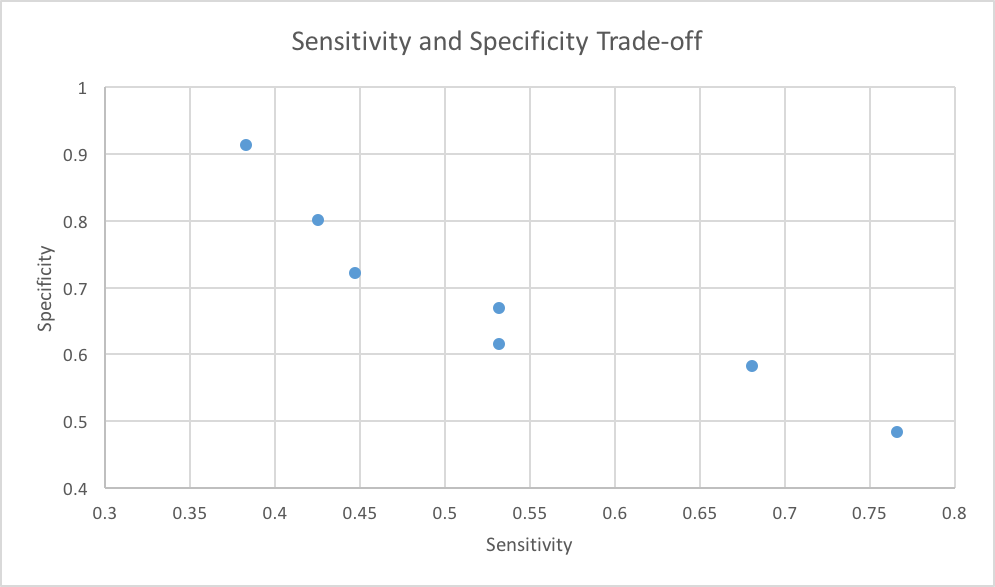
\includegraphics[scale=.7]{tradeoff.png}
\end{figure}

From the plot, we observed that we could improve the sensitivity to 76.60\%, i.e. more than three fourth patients can be determined correctly who reveals their cancer. However, the specificity will drop to 48.34\%. 
{\it Semi-Supervised learning discussion}
During the real-time implementation, we observe that the semi-supervised learning doesn't reach the improvements as we expected. The test error doesn't have observable enhancement after we incorporate the training related to unlabeled data. According to Xiaojin's Paper, there are three assumptions when applying semi-supervised learning: \\
1. Smoothness assumption: Points which are close to each other are more likely to share a label. \\
2. Cluster assumption: The data tend to form discrete clusters, and points in the same cluster are more likely to share a label. \\
3. Manifold assumption: The data lie approximately on a manifold of much lower dimension than the input space.\\

However, from the scratch plot (Figure 1) as an example, we observed that there is no strong evidence to support Smoothness assumption and Cluster assumption. That is why the semi-supervised learning method doesn't give us significant improvement.

\subsubsection*{References}

\small{
[1] Diana Dumitru. "Prediction of recurrent events in breast cancer using the Naive Bayesian classification" {\it Annals of University of Craiova} (2009), Vol 36(2).

[2] Chapelle, Olivier; Sch�lkopf, Bernhard; Zien, Alexander (2006). {\it Semi-supervised learning.}
Cambridge, Mass.: MIT Press.�ISBN�978-0-262-03358-9.

[3]  Zhu, Xiaojin.�{\it Semi-Supervised Learning}�University of Wisconsin-Madison.

[4] K. Nigam, A. K. McCallum, S. Thrun, and T. Mitchell. {\it Text classification from labeled and unlabeled documents using EM. Machine Learning}, 39(2/3):103-134, 2000.

\end{document}
